\section{Rectilinear Planar Embedding}

\subsection{Exercise 2.1}

Table \ref{tab:Xvf} shows the values for {\(x_{vf}\)} that correspond to Figure 3 from the Assignment Document.

\begin{table}[h]
  \centering
  \begin{tabular}{l | l l l l l}
  \(x_{vf}\) & a & b & c & d  & e  \\
  \hline
  \(v_{1}\)  & 0 & 1 & 1 & 0  & 0  \\
  \(v_{2}\)  & 0 & 0 & 1 & 1  & 0  \\
  \(v_{3}\)  & 1 & 0 & 1 & 1  & 1  \\
  \(v_{4}\)  & 0 & 0 & 0 & -1 & 1  \\
  \(v_{5}\)  & 1 & 0 & 0 & 0  & -1 \\
  \(v_{6}\)  & 1 & 1 & 0 & 1  & 1  \\
  \(v_{7}\)  & 0 & 0 & 0 & 0  & 0
  \end{tabular}
  \caption{\(x_{vf}\) values for Figure 3 in Assignment Document}
  \label{tab:Xvf}
\end{table}


Table \ref{tab:Zvf} shows the values for \(z_{fg}\) that correspond to Figure 3 from the Assignment Document. There are 13 break-points in this graph.
\begin{table}[h]
  \centering
  \begin{tabular}{l|lllll}
  \(z_{fg}\) & a & b & c & d & e \\\hline
  a     & - & 0 & 0 & 0 & 0 \\
  b     & 2 & - & 1 & 1 & 0 \\
  c     & 1 & 1 & - & 0 & 0 \\
  d     & 0 & 1 & 0 & - & 1 \\
  e     & 4 & 0 & 0 & 0 & - \\
  \end{tabular}
  \caption{\(z_{fg}\) values for Figure 3 in Assignment Document}
  \label{tab:Zvf}
\end{table}

We are asked to draw a rectilinear layout of graph 2(a) from the assignment description
\begin{figure}[ht]
  \centering
  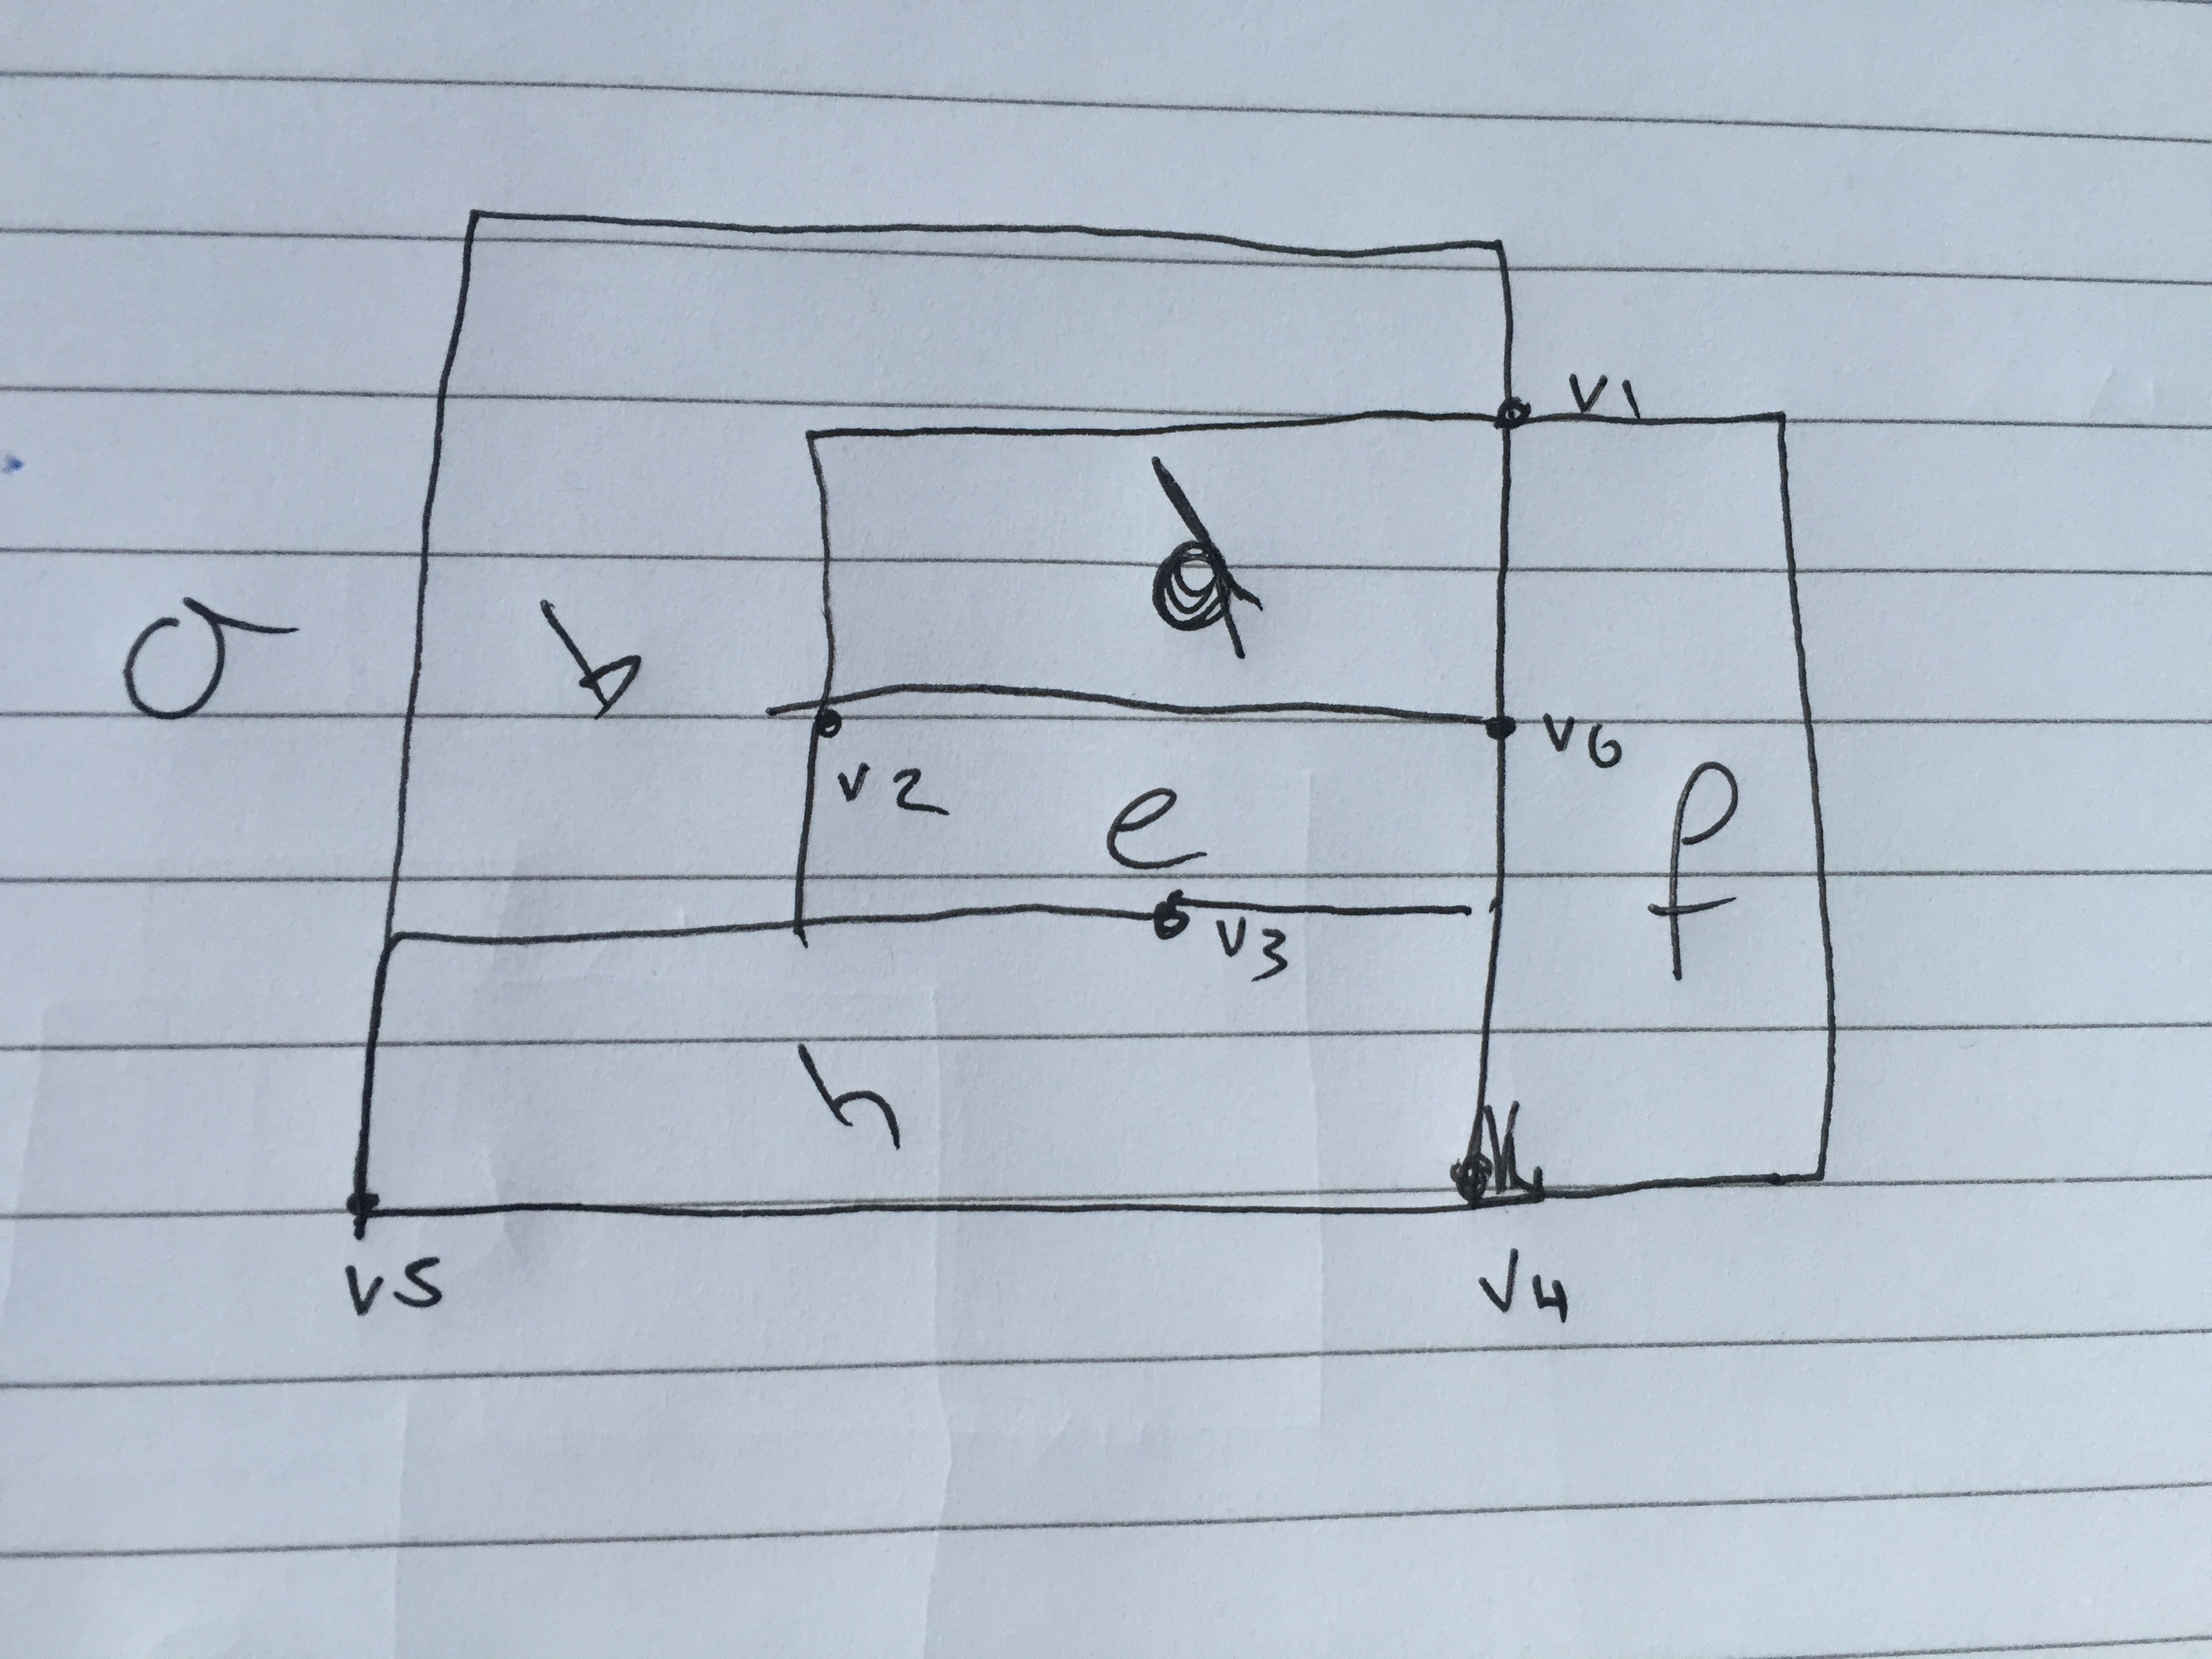
\includegraphics[scale=0.07]{images/planar-drawing.png}
  \caption{Rectilinear drawing of Graph 2(a) in assignment desc}
  \label{fig:rectidraw}
\end{figure}

\subsection{Exercise 2.2}
Let \(f_e\) be the external boundary cycle and \(F\) be the set of all boundary cycles. Given two boundary cycles \(x\) and \(y\), inner turns (from \(x\) to \(y\)) are denoted by \(z_{xy}\) and outer turns (from \(y\) to \(x\)) are denoted by \(z{yx}\).
\begin{align}
  \sum_{v} x_{vf_{e}} +&\, \sum_{b\in F \backslash {f_e}} z_{f_{e}b} - z_{bf_{e}} =& -4\\
  \forall b \in F \backslash {f_e}:\sum_{v} x_{vf} +&\, \sum_{b\in F \backslash {f}} z_{fb} - z_{bf} =& 4
\end{align}

Boundary cycle \(a\) is the external boundary cycle so Equation 3 must hold.
\[ \sum_{v} x_{v a} + \sum_{b\in B\setminus \{a\}} z_{a b} - z_{b a} \]
\[=  3 + z_{ab} - z_{ba} + z_{ac} - z_{ca} + z_{ad} - z_{da} + z_{ae} - z_{ea} \]
  \[=  3 + 0 - 2 + 0 - 1 + 0 - 0 + 0 - 4 \]
  \[=  3 - 2 - 1 - 4 = -4\]
%%
Boundary cycle \(e\) is an internal boundary cycle so Equation 4 must hold.

  \[ \sum_{v} x_{vf} + \sum_{b\in B\setminus f} z_{fb} - z_{bf} \]
  \[= 2 + z_{ea} - z_{ae} + z_{eb} - z_{be} + z_{ec} - z_{ce} + z_{ed} - z_{de} \]
 \[= 2 + 4 - 0 + 0 - 0 + 0 - 0 + 0 - 2 \]
 \[= 2 + 4 - 2 = 4 \]

\subsection{Exercise 2.3}
Since G is a graph that contains only straight and horizontal edges, it is impossible for G to have more than 4 edges: a horizontal edge going left; a horizontal edge going right; a vertical edge going up; a vertical edge going down. To show that Equation 1 from the Assignment Document holds we will show that it is true for each of the 3 cases presented, ie \(v\) has degree \(\in [2,3,4]\).

Firstly, the sum of the angles for a vertex \(v\) must equal 360\(^\circ\). Secondly, as we only allow horizontal and vertical edges the only possible turn angles \(\in [90,180,270] \) for an \(x_{vf}\). We will use these fact to show that the conditions hold for each of the three cases presented.

Case 1: \(v\) has degree 2.\newline
Then there are exactly 2 boundary cycles that pass through \(v\), say \(h\) and \(g\). Then there are only two possible combinations of the inner and outer turns from the point of view from each boundary cycle. Either both are 180\(^\circ\), and therefore \( x_{vh} = 0 \) and  \( x_{vg} = 0 \). So \(\sum_f x_{vf} = 0 \). Or one boundary cycle has a turn of 90\(^\circ\) (an inner turn, \(x_{vf'} = 1\)) and the other a turn of 270\(^\circ\) (an outer turn,  \(x_{vf''} = -1\)), then \(\Sigma_f x_{vf} = 1 - 1 = 0 \)

Case 2: \(v\) has degree 3.\newline
Then there are exactly 3 boundary cycles that pass through \(v\), then since the angles around \(v\) must add to 360\(^\circ\) and we can only have horizontal or vertical edges then there must be one angle of 180\(^\circ\) and two 90\(^\circ\) turns, thus there can only be two inner turns and  \(\sum_f x_{vf} = 0 + 1+ 1= 2 \)

Case 3: \(v\) has degree 4.\newline
Then there are exactly 4 boundary cycles that pass through \(v\), as the angles around \(v\) must add to 360\(^\circ\),  we can only have four 90\(^\circ\) turns, thus there can only be four inner turns and  \(\sum_f x_{vf} = 1 +1 + 1+ 1= 4 \)

\subsection{Exercise 2.4}
The objective function is given by \[min \sum_{\forall f \in G, f \neq g} z_{fg}\] given that the aim is to minimise the number of break points. The constraints that the problem is subjected to are:
\begin{align}
  &z_{fg}, z_{gf}& \geq& 0\\
  &\sum_{v} x_{vf_{e}} + \sum_{b\in F \backslash {f_e}} z_{f_{e}b} - z_{bf_{e}}& =& -4\\
  &\forall b \in F \backslash {f_e}:\sum_{v} x_{vf} + \sum_{b\in F\backslash {f}} z_{fb} - z_{bf}& =& 4\\
  & \sum_f x_{vf} & =&
  \begin{cases}  
    0 & \text{if \(v\) has degree \(2\)}\\
    2 & \text{if \(v\) has degree \(3\)}\\
    4 & \text{if \(v\) has degree \(4\)}
  \end{cases}
\end{align}

\subsection{Exercise 2.5}
Given a rectilinear graph \(G = (V,E)\) and a MCFP \(G' = (V',E')\). V'  is the set of vertices which contains all vertices \(v \in G\), and also a vertex for every face in \(G\).  \(E'\) is the set of edges which contains edges \((f,g)\) for f,g faces in \(G\) , if f and g share a vertex, and edges \((v,f)\) for \(v \in V\) if v was a vertex in f. As we are dealing with turns and breakpoints, and these are relative to faces and vertices and faces and faces, there is no information stored on connections from vertices to vertices in \(G\) and therefore these connections are not present in \(G'\). The \(z_{fg}\) variables.

The transformation from a rectilinear graph to a MCFP is given by the following conditions:
\begin{quote}
  \begin{itemize}
    \item{} \((v,f)\) where vertex v lies on the boundary of face \(f\) in \(G\). The capacity of these
        edges is lower bounded by 1 and upper bounded by 4. They have zero cost.
    \item{} \((f,g)\) and \((g,f)\) for every pair of adjacent faces, \(f\) and \(g\) in \(G\). The capacity of these edges is lower bounded by 0 and upper bounded by infinity. They have unit cost.
  \end{itemize}
  \flushright{\citep{drawings}}
\end{quote}

Given the above our graph solution to this question is based on the assumption that two faces \(f\) and \(g\) are adjecent if they share a vertex \(v\). This assumption yields the following sets of connected vertices:

\begin{align}
  &a:& {v_1, v_4, v_5, b, c, d, f, g h}\\
  &b:& {v_1, v_2, v_5, a, c, d, e, h}\\
  &c:& {v_2, v_3, v_5, a, b, d, e, h}\\
  &d:& {v_1, v_2, v_6, a, b, c, e, g, f}\\
  &e:& {v_2, v_3, v_6, b, c, d, f, g, h}\\
  &f:& {v_1, v_4, v_6, a, d, e, g, h}\\
  &g:& {v_3, v_4, v_6, a, d, e, f, h}\\
  &h:& {v_3, v_4, v_5, a, b, c, e, f, h}
\end{align}

% \begin{tikzpicture}
%   [scale=0.8,auto=left]
%   \tikzstyle{every node}=[shape=circle,fill=white,draw=black,text=black]
%   % Faces
%   \node (fa) at (1,10) {a};
%   \node (fb) at (4,8) {b};
%   \node (fc) at (5,2) {c};
%   \node (fd) at (5,6) {d};
%   \node (fe) at (3,4) {e};
%   \node (ff) at (9,1) {f};
%   \node (fg) at (7,10) {g};
%   \node (fh) at (8,10) {h};
%
%   % Vertices
%   \node (v1) at (1,1) {\(v_1\)};
%   \node (v2) at (3,2) {\(v_2\)};
%   \node (v3) at (5,3) {\(v_3\)};
%   \node (v4) at (7,4) {\(v_4\)};
%   \node (v5) at (9,5) {\(v_5\)};
%   \node (v6) at (1,6) {\(v_6\)};
%
%   % Connections from a
%   \foreach \from/\to in {fa/fb,fa/fh,fa/ff,fa/fc,fa/fg,fa/fd}
%     \draw (\from) -- (\to);
%
%   \foreach \from/\to in {v1/fa,v5/fa,v4/fa}
%     \draw (\from) -- (\to);
%   
%   % Connections from b
%   \foreach \from/\to in {fb/fd,fb/fc,fb/fe,fb/fh}
%     \draw (\from) -- (\to);
%
%   \foreach \from/\to in {v1/fb,v2/fb,v5/fb}
%     \draw (\from) -- (\to);
%   
%   % connections from c
%   \foreach \from/\to in {fc/fd,fc/fe,fc/fh}
%     \draw (\from) -- (\to);
%
%   \foreach \from/\to in {v2/fc,v3/fc,v5/fc}
%     \draw (\from) -- (\to);
%
%   % Connections from d
%   \foreach \from/\to in {fd/fe,fd/fg,fd/ff}
%     \draw (\from) -- (\to);
%
%   \foreach \from/\to in {v1/fd,v2/fd,v6/fd}
%     \draw (\from) -- (\to);
%
%   % Connections from e
%   \foreach \from/\to in {fe/ff,fe/fg,fe/fh}
%     \draw (\from) -- (\to);
%
%   \foreach \from/\to in {v2/fe,v3/fe,v6/fe}
%     \draw (\from) -- (\to);
%
%   % Connections from f
%   \foreach \from/\to in {ff/fg,ff/fh}
%     \draw (\from) -- (\to);
%   \foreach \from/\to in {v1/ff,v4/ff,v6/ff}
%     \draw (\from) -- (\to);
%
%   % Connetions from g
%   \foreach \from/\to in {fg/fh}
%     \draw (\from) -- (\to);
%
%   \foreach \from/\to in {v3/fg,v4/fg,v6/fg}
%     \draw (\from) -- (\to);
%
%   % Connections from h
%   \foreach \from/\to in {v3/fh,v4/fh,v5/fh}
%     \draw (\from) -- (\to);
% \end{tikzpicture}
